% summerSHG - technical notes
% to be posted to the CGP logbook
% should contain: how TL works, characterisation of TL, jitter noise floor discussion
% should not contain: timeline or mistakes, just useful results and methodology (if pertinent to replication)

\documentclass[aps,pra,superscriptaddress,reprint,nofootinbib]{revtex4-1}
% \documentclass[prb,reprint,nofootinbib]{revtex4-1} 
% \documentclass[pra,superscriptaddress,reprint,nofootinbib]{revtex4-1}
% \documentclass[prb,preprint,letterpaper,noeprint,longbibliography,nodoi,footinbib]{revtex4-1} 

% worry about formatting AFTER the text is written

\usepackage[utf8]{inputenc}
\usepackage{amsmath,amssymb,amsthm}
\usepackage{amsfonts}
\usepackage{graphicx}
\usepackage{float}
\usepackage{mathtools}
\usepackage[usenames,dvipsnames]{xcolor}	
\usepackage{hyperref}
% \usepackage{siunitx}
\usepackage{textcomp}
% \usepackage{subfiles}
\usepackage{comment}
% \usepackage[bottom]{footmisc}
% \usepackage{subfig}
% \usepackage[style=base]{caption}
\usepackage[caption=false]{subfig}

\usepackage{silence}
\WarningFilter{revtex4-1}{Repair the float}

%\bibliographystyle{apsrev4-2}
%\setlength{\parindent}{0pt}

% \newcommand{\abs}[1]{\left\lvert #1 \right\rvert}
% \newcommand{\norm}[1]{\left\lVert #1 \right\rVert}
% \newcommand{\ip}[2]{\langle #1,#2 \rangle}
% \newcommand{\expect}[1]{\langle #1 \rangle}

% \newcommand{\code}[1]{\texttt{#1}}
% \newcommand{\jam}[1]{\textcolor{magenta}{\textbf{#1}}}


\begin{document}
\title{Tilt locking the OPO - Technical notes}

\author{James W. Gardner}
\email{u6069809@anu.edu.au}
\affiliation{Centre for Gravitational Astrophysics, The Australian National University, Acton, A.C.T., 2601, Australia}
\affiliation{OzGrav @ ANU, Australian Research Council Centre of Excellence for Gravitational Wave Discovery, Acton, A.C.T., 2601, Australia}

\author{Min Jet Yap}
% \email{vaishali.adya@anu.edu.au}
\affiliation{Centre for Gravitational Astrophysics, The Australian National University, Acton, A.C.T., 2601, Australia}
\affiliation{OzGrav @ ANU, Australian Research Council Centre of Excellence for Gravitational Wave Discovery, Acton, A.C.T., 2601, Australia}

% \author{David McClelland}
% % \email{david.mcclelland@anu.edu.au}
% \affiliation{Centre for Gravitational Astrophysics, The Australian National University, Acton, A.C.T., 2601, Australia}
% \affiliation{OzGrav @ ANU, Australian Research Council Centre of Excellence for Gravitational Wave Discovery, Acton, A.C.T., 2601, Australia}

% \author{Sheon Chua}
% % \email{vaishali.adya@anu.edu.au}
% \affiliation{Centre for Gravitational Astrophysics, The Australian National University, Acton, A.C.T., 2601, Australia}
% \affiliation{OzGrav @ ANU, Australian Research Council Centre of Excellence for Gravitational Wave Discovery, Acton, A.C.T., 2601, Australia}

\date{\today}


%%%%%%%%%%%%%%%%%%%%%%%%%%%%%%%%%%%%%%%%%%
% \begin{abstract}
% % single paragraph, short sales pitch
% \end{abstract}

\maketitle

%%%%%%%%%%%%%%%%%%%%%%%%%%%%%%%%%%%%%%%%%%
\section{Preamble}
\label{sec:preamble}

These notes are written as a technical reference for the CGA squeezer group and assume an appropriate level of familiarity with the squeezer OPO table and any relevant concepts.
These notes do not give a chronological account of our work nor do they contain everything we attempted. For further information see the ``tilt locking'' series of posts in the CGP Logbook~\footnote{\url{http://chimera1.physics.anu.edu.au/wordpress/?tag=tilt-locking}} or contact the authors.

\subsection{Contents}

This Section~\ref{sec:preamble} serves an administrative and reference purpose.
Section~\ref{sec:TL} motivates, explains, and details our implementation of tilt locking (TL).
Section~\ref{sec:error_signal} gives a guide to improving the error signal of the TL control system.
Section~\ref{sec:out-of-loop_sensors} motivates and details the out-of-loop sensors that we used to characterise the TL control system.
Section~\ref{sec:results} contains miscellaneous results that characterise the TL control system and compare its performance to the PDH control system previously implemented.
And Section~\ref{sec:conclusions} draws conclusions about the efficacy of the TL control system.


%%%%%%%%%%%%%%%%%%%%%%%%%%%%%%%%%%%%%%%%%%
\section{Tilt locking (TL)}
\label{sec:TL}

\subsection{Motivation}

For squeezing experiments down the beam line, we want to keep the OPO on resonance to maximise the laser power inside the cavity. Whether the cavity is on resonance (considering just plane waves for the moment) depends on the laser frequency and the cavity tuning. Here, we are trying to lock the cavity length as to stay on resonance for the fundamental spatial mode. Note that we will refer to cavity tuning interchangeably as cavity length (e.g. length noise) throughout these notes which may be confusing if one insists that length be restricted to integer multiples of the carrier wavelength.


The OPO table already had a PDH control system in place to perform this function. One purpose of this work was to compare that existing system (PDH) to an alternative control system (tilt locking, see below). 


\subsection{Optics theory for TL}

This understanding and implementation is based off the work in Ref.~\cite{TL:1999}, see that reference for further information.


Classically, the laser light incident on the cavity can be decomposed into the Hermite-Gauss (HG) rectangular modes. How much the cavity is detuned determines how it ``sees'' these modes. Critically, the different spatial structure of these modes gives each a different Gouy phase that implies a different resonance condition (length/tuning) for each mode. As such, at different detunings the cavity will ``see'' different modes as resonant.


We restrict our attention to the fundamental (a single blob) and the first-order (two blobs side-by-side either vertically or horizontally along the two transverse x and y axes, respectively) HG modes. We placed a quadrature photodiode (QPD) to detect the light reflected off of the cavity such that the quadrature axes were (roughly) aligned with the horizontal and vertical transverse axes of the beam. The QPD outputs SUM, YDIFF, and XDIFF channels for the total intensity and the difference in intensity on the horizontal and vertical halves, respectively. If either mode is incident on the QPD alone, then the DIFF signals are zero (supposing that it is properly aligned). But if the fundamental and a first-order mode are both present at the QPD, then their interference will produce a non-zero DIFF signal for the relevant axis.


Putting these concepts together, when the cavity is on resonance for either the fundamental or the first-order mode, the DIFF signal is zero as that mode is not at the QPD to interfere with (\textbf{check this}). Then, for detuning close to resonance, the DIFF signal response is approximately linear with the cavity tuning. Tilt locking uses this linear response near the zero-crossing associated with the fundamental resonance as its error signal for controlling the cavity length by driving a PZT behind one of the cavity mirrors.


\subsection{Implementation}

% layout

% For the TL path, place lenses before steering mirrors if possible, else their behaviour can be unpredictable

% Throughout we used an oscilloscope for monitoring and a SR785 for LF (100 kHz down) measurements

\begin{figure*}
	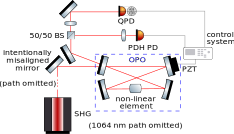
\includegraphics[height=0.6\textwidth,angle=-90]{figures/TL_layout.pdf}
	\caption{Schematic for tilt lock layout for cavity length control with PDH as an out-of-loop sensor.}
\end{figure*}


\subsection{Achieving lock}

With the system in place as above, including the HV amp on, to achieve lock the system must be manually guided to the linear regime of the error signal (manual lock acquisition) by use of the DC offset knob on the servo panel. Monitoring the QPD SUM and YDIFF signals on the oscilloscope, the user must slowly change the DC offset until the QPD SUM dips down and the error signal nears zero (signs of nearing a resonance). Then, quickly, the user must switch on the proportional (labelled as “signal”) and integral control. If the lock is successful, then the YDIFF error signal should remain at zero and disturbances such as clapping or stomping nearby can be seen on the trace.


However, it is likely that lock will not be initially achieved. The YDIFF error signal may need to be improved by the methods detailed in the below Section~\ref{sec:error_signal}. Alternatively, the servo gain may be too low and should be increased. If failure to lock is due to the lock finding the high-order resonance instead of the fundamental, then the user must reset and try again. If the system appears to be ringing while in lock or is losing lock due to ringing, then the servo gain should be turned down.


%%%%%%%%%%%%%%%%%%%%%%%%%%%%%%%%%%%%%%%%%%
\section{Improving the error signal}
\label{sec:error_signal}

\subsection{Intentional misalignment into the cavity}

% really improves the error signal but also increases the first-order resonance peak in the QPD SUM channel, do not over do else the control system could lock to the wrong resonance.


\subsection{Putting the lid on}


\subsection{Increasing the spot size}

% lens placement

\subsection{Dark and jitter noise}

% path length affects jitter noise


%%%%%%%%%%%%%%%%%%%%%%%%%%%%%%%%%%%%%%%%%%
\section{Out-of-loop sensors}
\label{sec:out-of-loop_sensors}

To characterise the TL control system, we introduced out-of-loop sensors to monitor the system.

\subsection{Theory of sensor noise}

\begin{figure}
	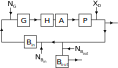
\includegraphics[height=0.5\textwidth,angle=-90]{figures/FCS_diagram.pdf}
	\caption{Block diagram for a SISO feedback control system with an out-of-loop sensor, $B_{\mathrm{out}}$. $B_{\mathrm{in}}$ is the in-loop sensor, $G$ is the compensator, $H$ is the driver, $A$ is the actuator, $P$ is the plant. The disturbance upon the free-running variable is $X_d$, the sensor noises are $N_{B_{i,o}}$, and the compensator noise is $N_G$.}
\end{figure}


This understanding is based of the introduction to control theory provided by Refs.~\cite{Ward:2010,Bechhoefer:2005,FCS:2000}.


Consider a simple SISO (single-input single-output) feedback loop working to suppress the disturbance to some variable in the system (as opposed to tracking a reference signal). The sensor observes the variable and produces an error signal for the compensator, which commands the driver-actuator to act on the plant as to make the error signal zero. Noise enters the system at three points, the free-running disturbance to the variable, at the sensor, and at the compensator. Note that while a priori noise could enter elsewhere in the system, these are the dominant sources~\cite{FCS:2000}. 


The free-running disturbance is suppressed at the control output (the same signal is input to the sensor) by the open-loop gain. If the gain is high enough such that the noise at the sensor (which does not change with gain) becomes dominant, then the sensor will start (unknowingly) treating it as a true disturbance to the system and will cause the plant to act on the system as to counter it, thereby introducing so called ``sensor noise'' into the system that the control loop is meant to be quieting. Further increasing the gain only injects more of this noise into the system. Sensor noise represents a limit to the efficacy of a control system since the sensor cannot distinguish its own noise from that in the physical system.


The tricky part of sensor noise, however, is that at the sensor output it is suppressed by the open-loop gain and so will not readily appear in any data using the sensor itself. To solve this and observe the sensor noise, a second, out-of-loop, sensor is added to complement the existing in-loop sensor. This out-of-loop sensor is only used for monitoring the system and its error signal is not fed back to any control system. Supposing that the out-of-loop sensor’s own noise is not louder than the in-loop sensor’s noise, then in regions of high gain where sensor noise is injected into the system the error signal from the out-of-loop sensor should hit a noise floor that cannot be passed by increasing gain. Meanwhile, the in-loop sensor would erroneously show better and better error signals.


\subsection{XDIFF (or the other TL channel)}


\subsection{PDH}


\subsubsection{Mixer noise}

We were surprised at the features in the PDH dark noise and that it was higher than the TL dark noise. We tracked this down to the old mixer euroboard used. We replaced it with a Minicircuits ZP-3+ with an attached LP filter, which improved and flattened the dark noise and also allowed for some attenuation to be removed.


%%%%%%%%%%%%%%%%%%%%%%%%%%%%%%%%%%%%%%%%%%
\section{Results}
\label{sec:results}

\subsection{Open-loop gain}


\subsection{Jitter sensor noise}



%%%%%%%%%%%%%%%%%%%%%%%%%%%%%%%%%%%%%%%%%%
\section{Conclusions}
\label{sec:conclusions}



%%%%%%%%%%%%%%%%%%%%%%%%%%%%%%%%%%%%%%%%%%
\nocite{*}
\bibliographystyle{myunsrt}
\bibliography{technical_notes}


\end{document}
